\chapter{Preliminary Study}

\section{Concept}

\section{Constraints}
\subsection{Time}
The project must be completed within a timeframe of 13.6 weeks. The guideline is 24.3 work hours per person, per week. 
\subsection{Knowledge about the problem}
Our problem is not well-explored and the customer cannot give us exact requirements. Thus, this is as much a research project as it is a software development project.

\section{Feasibility study}

\section{Similar solutions}

\subsection{Counter-Strike}

\begin{wrapfigure}{r}{.275\textwidth}
\vspace{-30pt}
\centering
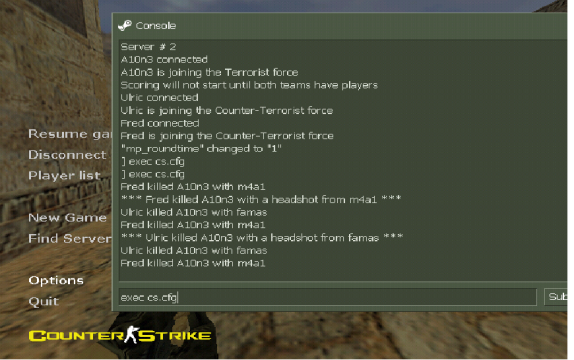
\includegraphics[width = .25\textwidth]{image/counterstrike.png}
\end{wrapfigure}

This game features a console that offers a wide variety of commands, including:
- Changing the game options
- Altering the game world
- Player actions and cheats
- Multiplayer communication and administration

In a game, this functionality eases development and debugging, as well as increasing the moddability and long-term value for players. Similar consoles also exist in other games, such as Carmageddon TDR 2000.

\subsection{Blender}

\begin{wrapfigure}{r}{.275\textwidth}
\vspace{-30pt}
\centering
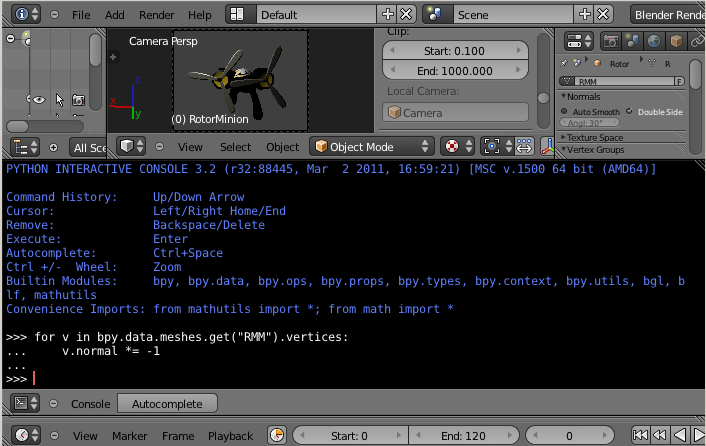
\includegraphics[width = .25\textwidth]{image/blender.png}
\end{wrapfigure}

This 3D modelling software features a Python console with access to the model data, animation data, etc. It can be used to perform operations that are not directly supported in the user interface. It is also common to extend the program using custom Python scripts. 

Similar solutions also exist in other creative tools, including a Python console in GIMP and Nyquist prompt in Audacity.

\subsection{Firefox}

\begin{wrapfigure}{r}{.275\textwidth}
\vspace{-30pt}
\centering
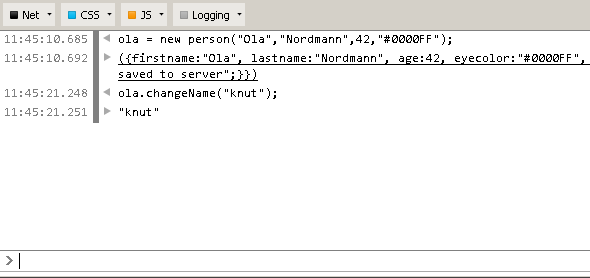
\includegraphics[width = .25\textwidth]{image/firefox.png}
\end{wrapfigure}

This web browser features a Web Console where it is possible to execute JavaScript commands with access to the objects on the current page. This is useful for web development and debugging. Similar features also exist in a few other browsers, such as Google Chrome.

\subsection{try.mongodb.org}

\begin{wrapfigure}{r}{.275\textwidth}
\vspace{-30pt}
\centering
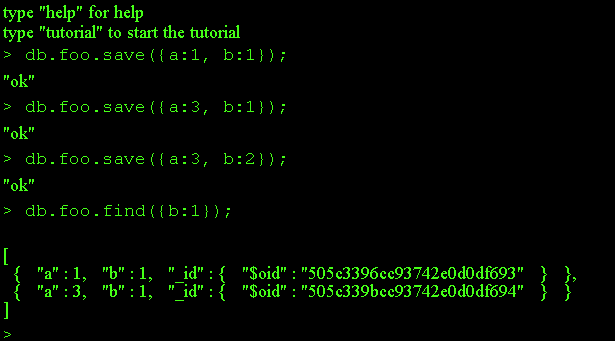
\includegraphics[width = .25\textwidth]{image/mongodb.png}
\end{wrapfigure}

This database website features a console where the user can execute commands on a dummy database. It is an educational tool for people who don't want to invest too much time in it. Comparable consoles also exist to allow the user to execute arbitrary queries in database administration tools such as PHPMyAdmin.

\subsection{web-console.org}

\begin{wrapfigure}{r}{.275\textwidth}
\vspace{-30pt}
\centering
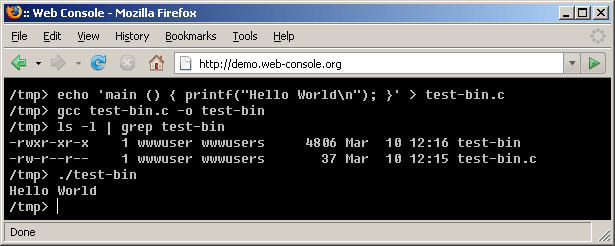
\includegraphics[width = .25\textwidth]{image/webconsole.png}
\end{wrapfigure}

This project provides shell access to a server through the browser window over HTTP.

It supports real time communication, and is intended to be used for server administration purposes.

\subsection{Conclusion}

This is by no means an exhaustive list, but it serves to illustrate that consoles are still applicable for purposes including software development, debugging, learning, extendability and where there is a high demand for flexibility.



\section{Version control}
\subsection{git}

\section{Development language and technologies}


\subsection{Client-side web application technologies}
Our main focus will be on the client part of the application, since this is the experimental part of our system, and it is this part that is visible to the user through the web browser. It is therefore important to choose a suitable technology for this.

\subsubsection{Adobe Flash}

\begin{wrapfigure}{r}{.15\textwidth}
\vspace{-30pt}
\centering

\includegraphics[width = .10\textwidth]{image/flash-logo.png}
\end{wrapfigure}


A multimedia platform currently owned by Adobe. Is currently the industry standard for multimedia web applications. It excels at animation and 2D games, but its strong points are not likely to be useful in our project. A separate JavaScript is required to perform communication with a server and the development tools are costly.

\subsubsection{Microsoft Silverlight}

\begin{wrapfigure}{r}{.15\textwidth}
\vspace{-47pt}
\centering
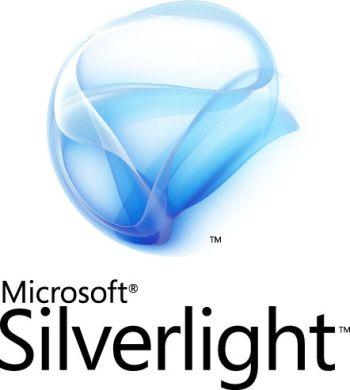
\includegraphics[width=.10\textwidth]{image/silverlight-logo.jpg}
\end{wrapfigure}

A rich media application framework developed by Microsoft. Useful for multimedia applications, but likely not beneficial for our project.

\subsubsection{Java Applets}

\begin{wrapfigure}{r}{.15\textwidth}
\vspace{-30pt}
\centering

\includegraphics[width=.14\textwidth]{image/java-logo.jpg}
\end{wrapfigure}

A technology that allows a Java AWT/Swing application to be displayed in a browser, backed by a Java Virtual Machine. Has excellent performance compared to other popular client side browser technologies. A signed applet can also communicate with a server using traditional sockets. It is possible to embed a scripting engine(for instance JavaScript). However, development effort may prove to become excessively heavy.

\subsubsection{JavaScript}

\begin{wrapfigure}{r}{.15\textwidth}
\vspace{-20pt}
\centering
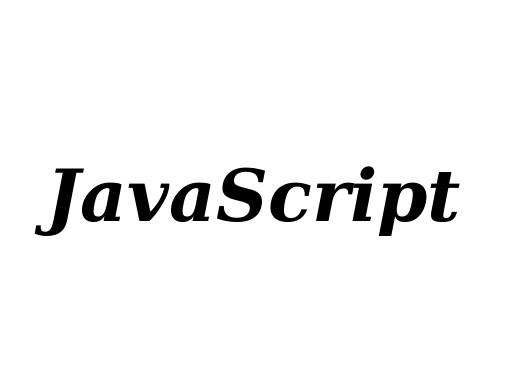
\includegraphics[width=.14\textwidth]{image/javascript-logo.png}
\end{wrapfigure}


JavaScript is a scripting language supported by all popular web browsers. Has extensive frameworks built around it and allows for rapid development. It is also possible to let the user write commands using JavaScript directly.

\subsubsection{Conclusion}
As a team, we have extensive experience with Java, and less with the other technologies. However, we all have at least some experience with JavaScript, and we believe that it is the better choice for this project: The DSL can be implemented by allowing the user to perform operations on the JavaScript objects using (a subset of) the JavaScript language itself. There are also excellent tools for transfer and storage of JavaScript objects. Furthermore, communication between JavaScript and HTML elements is easily achieved.

\subsubsection{JavaScript Related technologies}

\textbf{jQuery}\\*
A JavaScript library that simplifies how to use JavaScript to interact with the webpage, notably selection of Document Object Model elements.\\*
\\*
\textbf{MooTools}\\*
A JavaScript framework that, notably, enhances the Document Object Model and JavaScript's object oriented programming model.\\
\\*
\textbf{Dojo}\\*
A JavaScript toolkit offering asynchronous communication, a packaging system and systems for data storage. Intended to ease rapid JavaScript web development.\\*
\\*
\textbf{HTML5}\\*
A revision of the HTML standard currently still in development. Notably, it supplies support for multimedia and more advanced user interface elements. Is commonly used in conjunction with JavaScript.\\*
\\*
\textbf{CSS}\\*
Cascading Style Sheets, used to specify a consistent look and feel to a series of HTML documents.\\*


\subsection{Synchronization Technologies}
We will be adding a library for bi-directional real time communications between the server and the client, to easily detect changes in the objects on both sides and to replicate these changes to the other side lightning fast. This functionality will ensure data consistency between the client and server side. To make these updates fast and to avoid extra work in creating this functionality ourselves, we will employ an external library to get the work done.

\subsubsection{Pusher}

\begin{wrapfigure}{r}{.2\textwidth}
\centering

\includegraphics[width=.19\textwidth]{image/pusher-logo.jpg}
\end{wrapfigure}

Pusher is a cloud based system which offers a hosted API. It relies on the use of HTML5 WebSockets, which provides bi-directional communication over a TCP channel. It is a widely used solution which is well documented, and it support for a lot of libraries for both the server and client side. The web-site offers tutorials and extensive documentation on the most popular libraries. 

\begin{figure}
\centering
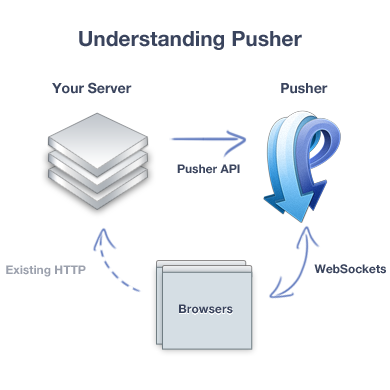
\includegraphics[width=3in]{image/pusher-explained.png}
\caption{Pusher Explained}
\end{figure}


Pusher creates channels that can be both listened and published to. If multiple devices are connected to the same channel, they will receive any messages sent to the channel almost simultaneously. Pusher offers a free account(an account is needed to use the system) which offers all the basic functionality we need, with up to 20 connections and 3 million messages per month

\subsubsection{PubNub}

\begin{wrapfigure}{r}{.2\textwidth}
\centering

\includegraphics[width=.19\textwidth]{image/pubnub-logo.png}
\end{wrapfigure}

Like Pusher, PubNub is a push service hosted in the cloud. It is written entirely in C, which gives it extremely fast performance and enables it to push over 1 million messages a second. It offers great documentation and support for the most popular libraries on both the client and server side and its in widespread use.

Like Pusher it relies on channels for communication which you can subscribe and publish to, and in essence the two solutions work in the same intuitive way. PubNub offers a free account with 1 million messages a month and up to 100 connections.

\subsubsection{Other Technologies}
We considered other similar alternatives as well, like Socket.io, Vert.x and Akka. But they either lacked support for the technologies we have chosen for the system, or lacked the extensive documentation and widespread use that Pusher and PubNub provides. We were also left with the impression that we would spend more time implementing these services than if we opted for either Pusher or PubNub.

\subsubsection{Conclusion}
Pusher and PubNub are both great systems that are widely used and they both offer extensive documentation. They cover the specific functionality we need for this project, which is to replicate the changes on both the client and server side. They both offer free accounts with more than enough connections and messages each month to cover our needs. So this decision will come down to our gut feeling. 

As none of the developers have any experience in using either system, the most important factor for this decision is that the system is well documented and easy to use. During research it became apparent that PubNub is the most widespread solution as of today. If we run into any problems implementing and using the system, it is likely someone has already provided a solution for it. So the decision ultimately fell on using PubNub.


\subsection{Markup Languages}
When communicating between the client and the server we need a data exchange format to represent objects and actions. The format has to be able to serialize and deserialize them on sending and receiving. The two alternatives most commonly in use today for solving this problem is XML (Extensive Markup Language) and JSON (JavaScript Object Notation).

\subsubsection{XML}
In widespread use in a lot of areas as of today and boasts great support and documentation. Originally meant to be a document markup language, but has over the years been used as a data representation language as well. It is suited to describe complex objects and documents, and it is easy to extend. Generally thought of as the more secure option of the two.

\subsubsection{JSON}
As the name suggest JSON is serialized JavaScript objects, well suited for web development, and very fast. JSON is easy for JavaScript to parse(we will be using JavaScript on both server and client), and the language has built in support for serializing and evaluating JSON data. Its small, simple, and easy to use. JSON is especially good at representing programming-language objects. It has gained a great deal of popularity in recent years, and it is well documented.

\subsubsection{Conclusion}
Both languages is well supported in almost all web related libraries, and they are both extensively documented. As security is not a main concern of this project, the fact that XML is more secure will not influence the decision

JSON will be used for this project. It covers the functionality we need, and it is generally thought of as the easier language to use. It is perfectly suited for web- development and JavaScript, which is the domain of this project. In addition the developers have more experience in using JSON than XML.

\subsection{Google Drive}

\section{Development Methodology}
\subsection{Agile vs Waterfall}
The waterfall method focus on planning the future in detail. It follows the principle of “Big Design Up Front”. It relies on the fact that you are able to report exactly what features that are going to be implemented and tasks are planned for the entire length of the project. It forces you to specify all the requirements early in the development, when you actually know the least about the project and the problems that are to be solved. The rationale behind this is that time spent early on making sure requirements and design are correct saves you much time and effort later. A development team using the waterfall method will only consider to implement the most valuable changes, as changes in this process are time consuming and often requires that completed work is started over. The method places a lot of emphasis on documentation. 

Agile methods, as opposed to the predictive methods, are designed to plan for changes in the requirements and features of a project. It emphasises on working code as primary measure of progress, instead of extensive documentation of for example the requirements. Agile methods consists of iterative and incremental steps in the development process, where requirements and solutions evolve through the course of the project. Requirements are bound to change, either because the customer didn't understand the problem in the beginning or because they would like to add new features. Agile methods facilitates the ability to accommodate these changes. Most agile methods includes delivering a working product in incremental stages, and gives the customer something to relate to during the developments process.

The CHAOS Manifesto is a survey published by the Standish Group each year and it measures the success of IT- projects. It divides the projects into 3 groups; Success, meaning it completed on time and budget, with all features and functions as specified. Challenged, meaning it  completed, but was over cost, over time, and/or lacking all of the features and functions that were originally specified. Failed, meaning the project was abandoned or cancelled at some point and thus became a total loss.

\begin{figure}
\centering
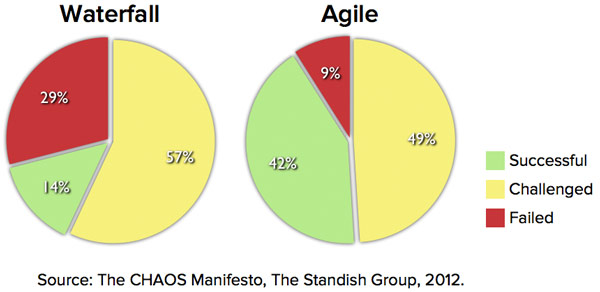
\includegraphics[width=3in]{image/Agile-Waterfall.jpeg}
\caption{Waterfall vs. Agile}
\label{figure:devchart}
\end{figure}

As the Figure~\ref{figure:devchart} illustrates, agile methods although not perfect by any means, more often result in products that are successful(the method used for measuring the success of a project is to some degree debated, but the results serves a purpose nevertheless).

\subsection{Agile Methods}
There exists a lot agile methods for software development, and although all of them follow the basic principles of agile development, they differ in a lot of areas. Following is a detailed description of three different agile methods.

\subsubsection{Scrum}
Scrum is an iterative, incremental software development model with several short sprints - complete small sets of tasks each sprint.

\begin{figure}
\centering
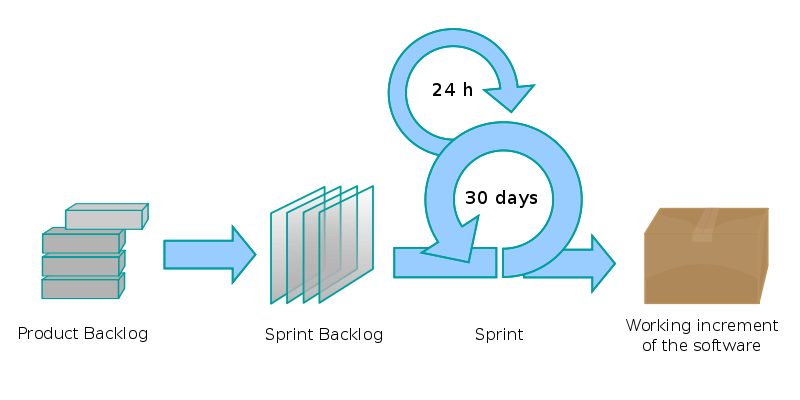
\includegraphics[width=4in]{image/Scrum_process.png}
\caption{Scrum Process}
\label{figure:devchart}
\end{figure}


The Roles: 
\begin{itemize}

\item The Scrum master, who is responsible for leading the process and to enforce the Scrum rules onto the team. He has to make sure that the development team does not overestimate what they can handle during one sprint. He leads the scrum meetings and enlightens and handles obstacles that may appear. 

\item The product owner, represents the stakeholders and is the voice of the customer.

\item The development team, is responsible for delivering potentially shippable product increments at the end of each Sprint. A development team is made up of 3–9 people with cross-functional skills.

\end{itemize}

The Sprints:
\begin{itemize}

\item Normally last from 7 to 30 days .
\item Starts with a planning meeting, where tasks are identified and goals for the sprint is set.
\item Product owner tells the team what tasks should be done in the sprint.
\item The tasks comes from a prioritized list of requirements called the backlog.
\item The team determines what is possible based on this and records this in a sprint backlog.
\item The goals should not be changed during the sprint.

\end{itemize}

The Scrum process is well suited for projects where its difficult to plan too far ahead, where at least some of the aspects of the project are unknown. Its a versatile process which is gives you the ability to handle changes in the requirements and demands from the customer. It allows for the developers to work on different parts of the project at the same time. The design, requirements of the system are not set in stone from the start, and are allowed to evolve during the process. The process delivers unfinished versions at the end of each sprint, which gives the customer a chance to try the system and give continuous feedback to the developers.

The Scrum process is somewhat complex, and it will take time to properly learn and execute the method. You also have to decide on what type of Scrum you are going to use, as there exists multiple forms of Scrum. This can prove to be a time consuming process. And even though the team members know Scrum, they will have to learn the version of scrum decided upon, if it turns out to differ from the one they are used to.
\footnote{\url{http://en.wikipedia.org/wiki/Scrum_(development)}}

\subsubsection{DSDM Atern}
DSDM(Dynamic System Development Method) is an agile software development method, and it was originally meant to provide some discipline to the Rapid Application Development method. The most recent version was launched in 2007 in an effort to make DSDM tool and technique independent, and its called Atern. 

DSDM is an iterative and incremental approach that embraces principles of agile development, including continuous user/customer involvement. It enforces you to deliver incremental versions of the product to the customer, where the main criteria of acceptance is that it meets the current business needs of the customer. It follows the principle that it is always better to deliver something “good enough” early than to deliver everything “perfect” in the end.

DSDM as a method fixes costs, quality and time at the beginning of the project. Through a prioritization method called the “MoSCoW Method”, with musts, shoulds, coulds and won’t haves, it adjusts the scope of the project to meet the given time frame. This allows the development team to focus on the critical functions of the system rather than delivering a perfect system. The method puts a strong focus on actively involving the customer in the development, and continually confirm the solution.

The principle-list of DSDM is quite long and complex. For a team that is not experienced in using the method, the process of learning the method will be time consuming. Also, always having to display the progress to the customer can be time consuming and hinder the development effort. 
Testing is central and shall be done through the whole development process.
\footnote{\url{http://en.wikipedia.org/wiki/DSDM}}

\subsubsection{Extreme Programming}
Extreme programming, hereby referred to as XP, is an agile method designed to reduce cost of changes in requirements by having multiple short development cycles. It includes elements such as pair- programming, extensive code review and unit testing of all the elements of the code. It emphasises frequent communication with the customer and between the developers.

The method embraces changes in the requirements of the project, and it doesn't attempt to define a stable set of requirements at the beginning of the project. In XP a representative for the customer is always available on site to answer any questions the developers might have. It also focuses on frequent releases of working code which serves as checkpoints where the customer can add new requirements.
 
XP puts a lot of focus on the code of the project, the advocates of XP argues that the code is the only truly important product of the system development process. XP as a process does not produce a lot of written documents during the development of the project. In XP programmers are expected to assume a unified client viewpoint and focus on coding rather than documentation of compromise objectives and constraints.
\footnote{\url{http://en.wikipedia.org/wiki/Extreme_Programming}}

\subsection{Conclusion}
If all of the requirements of this project were known in advance and provided by the customer, or the features of the finished product was known and unlikely to change, the waterfall method might be the way to go. But this is a prototype, proof of concept type of project where very little is known about the final product. We were certainly not presented with a finished set of requirements at the beginning of the project, and the requirements we settle on before we start the implementation are also more than likely to change during development. These kind of changes in a waterfall process will be time consuming. Thats why we think that an agile development method will be the best choice for this project.

All of the agile methods described above exhibits properties that will come in useful in this project. They are all based on iterative and incremental development steps, delivering prototypes for the customer to test after each step. This will give the customer a chance to try out unfinished versions of the product and give continuous feedback throughout the project. It can also help the customer to identify new features that they would like to add. They also allows the customer to decide which features to implement in each step, ensuring that the final product will contain the features the customer really need.

The agile methods embrace changes in the requirement and provides ways to handle those changes. They also encourage tight and continuous communication with the customer, which is important to be able to deliver a product that the customer is satisfied with

Of the three methods the group members are most familiar with the Scrum process. The DSDM method is complex and will take a considerable effort to learn and execute correctly. As none of the group members have used DSDM, and we have a limited amount of time in this project, DSDM is of the table. 

XP puts a lot of focus on the code, and delivers a minimal set of documents. We are to write an extensive report about the project, and document every part of it, including compromises and assumptions made. The amount of code in this project will be limited and none of the team members have any experience in working with XP. As a result, XP seems like a bad fit for our project.

The Scrum process does not put as much focus on documentation as the waterfall process, but we think that the amount of documentation produced during the Scrum process will be satisfactory for the report. It will take time to learn how to execute Scrum properly, but since all of the group members are familiar with the basics of process, we think it won’t be too time consuming and worth the effort. The final decision then is to use Scrum as a development method for this project.

\section{Software Testing}

\subsection{Testing Methods}
The purpose of software testing is to uncover software bugs in the system and to document that the system meet the requirements and functionality that was agreed upon for the system. Testing can be implemented at any stage in the development process, traditionally it is performed after the requirements have been defined and the implementation is completed. In agile development processes however, the testing is an ongoing process. The chosen development methodology will in most cases govern the type of testing implemented in a given project.

Software testing methods are traditionally divided into white- and black- box testing. They differ mainly in how the test engineer derives test cases.

\subsubsection{White- Box Testing}
White- box testing focus on the internal structures of a system, and it uses this internal perspective to derive test cases. White- box testing is usually done at unit level, testing specific parts or components of the code. This kind of testing focus on how something is implemented and not necessarily why. Unit testing alone cannot verify the functionality of a piece of software is supposed to exhibit. It can uncover many errors or problems, but it might not detect unimplemented parts of the specification or missing requirements.

\subsubsection{Black- Box Testing}
Black- box testing handles the software as a black- box, meaning it observes the functionality the system exhibits and not the specifics on how it is implemented. The tester only needs to be aware of what the program is supposed to do, he doesn't need to know the specifics on how the functionality is implemented in the code. Black- box testing is typically performed to check if the functionality of the program is according to the agreed upon requirements, both functional and nonfunctional. Black- box testing is usually done at the component, system and release levels of testing.

The main advantage of black- box testing is that no programming knowledge is needed to actually perform the tests. This way you can hire someone outside the development team who has had nothing to do with the implementation of the code to write and perform the tests, and you achieve as little ownership of the code as possible. An argument can be made though that this lack of insight in the specifics of the source code will result in repeated testing of some parts of the code, while other parts could be left untested.

\subsubsection{Test Driven Development}
The principle behind TDD is to develop the code incrementally, along with test for that increment. You don’t move on until the code passes its test. The tests are to be written before you actually implement the new functionality. The process helps programmers clarify their ideas of what a code segment is actually supposed to do. The process is often used in agile development methods.
Benefits from TDD include: 
\begin{itemize}

\item Code coverage, every code segment should be covered at least one test.

\item Regression testing, check to see if changes in the code have not introduced new bugs.

\item Simplified debugging, when a test fails it should be obvious where the problem lies, no need for a debug tool.

\item System documentation, the tests themselves act as a form of documentation that describe what the code should be doing.

\end{itemize}

\subsubsection{Automated Tests}
Automated offers the ability to automatically do regression tests, i.e. testing to uncover if any new code has broken a test that previously passed. If we opt for manual testing regression testing will be very time consuming as every test done so far has to be done over again. With an automated testing framework this job will be a lot easier as you can run a great number of tests in a matter of seconds. Most development languages offers libraries for automated testing.


\subsection{Testing Levels}
Testing can be done at many different levels and in different stages in the development process. Following is the most common partitioning of testing levels and a description on each of them.

\subsubsection{Unit Testing}
Unit testing aims to check specific components, such as methods and objects. Typically you will be testing objects, and you should provide test coverage of all the features of that object. Its important to choose effective unit test cases, that reflect normal operation and they should show that the specific component works. Abnormal inputs should also be included to check if these are processed correctly.

\subsubsection{Component Testing}
Tests bigger components of the system, and their interfaces(communication with other components). Made up of several interacting objects. Component testing is mainly a tool to check if component interfaces behaves according to its specification.

\subsubsection{System Testing}
In a given development project there may be several reusable components that have been developed separately and COTS systems, that has to be integrated with newly developed components. The complete system composing of the different parts is tested at this level. Components developed by different team members or groups may also be integrated and tested at this stage.

\subsubsection{Release Testing}
Release testing is the process of testing a particular release of the system that is intended for use outside of the development team. Often a separate team that has not been involved in the development perform this testing. These kind of tests should focus on finding bugs in the complete system. The objective is to prove to the customer that the product is good enough. This kind of testing could either be based on the requirements of the system or on user scenarios.

\subsubsection{User Testing}
This is a stage in the testing process in which users or customers provide feedback and advice. This could be an informal process where end- users experiment with a new system too see if they like it and that it conforms to their specific needs. Testing on end- users is essential for achieving success in a software process as replicating the exact working environment the system will be used in is difficult to achieve during development. The end users can help provide feedback on how specific functionality will work in an actual work environment.

Another form of user testing involves the customer and its called acceptance testing. Its a process where the customer formally tests a system to decide whether or not it should be accepted, where acceptance implies that payment for the system should be made. Acceptance testing is performed after the release testing phase.

\subsection{Conclusion}
The concept of TDD is to develop exhaustive tests that specify the system, and then writing code with the goal of satisfying the tests. This is useful in systems where the key functionality is in the form of program logic that can be verified to conform to the specification. It is difficult to write such exhaustive tests in applications that rely heavily on GUIs, network connections and database systems because of the added complexity and heterogeneousness that these features involve. In addition, our prototype's exact specifications are likely to change during development, requiring large amounts of test rewriting in the case of TDD, because the tests will be more numerous and because the tests must be more strict. As a result we have opted not to use TDD in this project. We will however be utilizing unit tests with an automated testing framework where it is appropriate and will harvest some of the advantages linked to TDD, like the automated regression testing.

We will be writing unit tests throughout the implementation process and run these continuously. These tests will not be included in the report as test cases. The test cases will rather comprise of component and system tests. Component tests will be used to test specific components and their functionality as well as their interaction with other components. System tests will be used on the system as a whole to check if it meets the agreed upon requirements. These test cases will be derived from the requirements. We will also try include some acceptance tests to include the customer in the testing process. 

We will be utilizing user testing and involve end users to get feedback on the entire system or specific functions. This testing will mainly be used to get feedback on the domain scripting language and how easy it is to understand and use. Preferably it will be done continuously throughout the development process. It is important to involve users as the goal of this project is to ease their workflow. As we are not working with an existing system thats actually in use, there will not exist any real users of this system with experience using it. We will therefore mainly be using our fellow students as test subjects, as they are readily available and technically competent enough to understand the concept and act as superusers. In addition the customer has stated that it will encourage employees from the entire company to us give feedback if we ask for it. Specific solutions can be sent to the customer representative which in turn will relay it to experts on the area it concerns.

\section{Code conventions}
\section{Similar solutions}